\subsection{Partial Differential Equations - Chapter 29}

\begin{enumerate}

  \item {\bf Overview of PDEs}

    All equations we've dealt with thus far involves functions of one
    dimension $f(t)$ (initial value problems) or $f(x)$ (boundary value
    problems). In engineering, problems are rarely one-dimensional and
    usually involve multiple independent variables $f(x,y,z,t)$
    (spatially and temporally varying wind field for example). Most
    systems encountered in engineering are second order and can be
    expressed using the equation below.

    \begin{equation} 
      A \frac{\partial^2 u}{\partial x^2} + B \frac{\partial^2
        u}{\partial x \partial y} + C \frac{\partial^2 u}{\partial y^2}
      + D = 0
    \end{equation}
    
    If $B^2-4AC < 0$ the equation is elliptic. If $B^2-4AC = 0$ the
    equation is parabolic and if $B^2-4AC > 0$ the equation is
    hyperbolic. 

  \item {\bf Elliptic Equations}

    The 2-D heat transfer governing equation is

    \begin{equation}
      k_x \frac{\partial^2 T}{\partial x^2} + k_y \frac{\partial^2
        T}{\partial y^2} + Q = \frac{2h}{t} (T-T_\infty)
    \end{equation}
    
    where $k$ is the thermal conductivity, $T$ is the temperature, $Q$
    is the heat source, $h$ is the convection coefficient and $t$ is
    the plate thickness. If the plate is insulated on its lateral
    surfaces(top and bottom), $k_x=k_y=k$ and $Q=0$, the governing equation becomes 

    \begin{equation}
      \frac{\partial^2 T}{\partial x^2} + \frac{\partial^2
        T}{\partial y^2} = 0
    \end{equation}
    
    In the general form this means that A = 1, B = 0, C = 1 and C = 0
    thus $B^2-4AC = -4 < 0$ which means the equation is elliptic. In
    order to solve this equation the system is discretized into a set
    of grid points. Then the partial derivatives can be approximated
    using central difference formulas.

    \begin{equation}
      \frac{T_{i+1,j} - 2T_{i,j} + T_{i-1,j}}{\Delta x^2} +
      \frac{T_{i,j+1} - 2T_{i,j} + T_{i,j-1}}{\Delta y^2} = 0
    \end{equation}

    If $\Delta x = \Delta y$ the equation reduces to 
    
    \begin{equation}\label{e:heat_equation2d}
      T_{i+1,j} + T_{i-1,j} + T_{i,j+1} - 4T_{i,j} + T_{i,j-1} = 0
    \end{equation}

    Assume you start with grid point $i=1$ and $j=1$. The equation is
    then

    \begin{equation}
      T_{2,1} + T_{0,1} + T_{1,2} - 4T_{1,1} + T_{1,0} = 0
    \end{equation}
    
    If boundary conditions are used such that $T_{0,j} = 75^o$,
    $T_{i,0} = 0^o$, $T_{4,j} = 50^o$ and $T_{i,4} = 100^o$ (assume a
    3x3 grid) the equation above reduces to

    \begin{equation}\label{e:heat_example}
      \begin{matrix}
      T_{2,1} + 75 + T_{1,2} - 4T_{1,1} + 0 = 0 \\
      T_{2,1} + T_{1,2} - 4T_{1,1}  = -75
      \end{matrix}
    \end{equation}

    Note that when boundary conditions are given this is known as
    Dirichlet boundary conditions, that is the temperature is held
    constant. If instead the sides are insulated it means the heat
    flux ($\partial T/\partial x$) is zero. Thus the derivative is
    given instead of the value. This is known as a Neumann condition. 

    Repeating equation \ref{e:heat_example} for all 9 grid points yields a system of
    the form $A\vec{x} = b$ where A is a 9x9 matrix. This can then be
    solved by any numerical solver just like the single dimension
    boundary value problem. 

    The solution is shown in the matrix below

    \begin{equation}
      T(x,y) = \begin{bmatrix} 43.0000   & 33.3000 &  33.8900 \\
        63.2100 &  56.1100 &  52.3400 \\
        78.5900 &  76.0600 &  69.7100 \\
      \end{bmatrix}
    \end{equation}
    
    This can be plotted in MATLAB using the function below

    \begin{framed}
      x = 1:3;
      
      y = 1:3;
      
      [xx,yy] = meshgrid(x,y);

      Tsolution = [43 33.3 33.89;63.21 56.11 52.34;78.59 76.06 69.71];

      mesh(xx,yy,Tsolution)

    \end{framed}

    Notice that MATLAB matrices are top to bottom so make sure you
    enter the solution in correctly otherwise you will get incorrect results.

    \begin{figure}[H]
     \begin{center}
       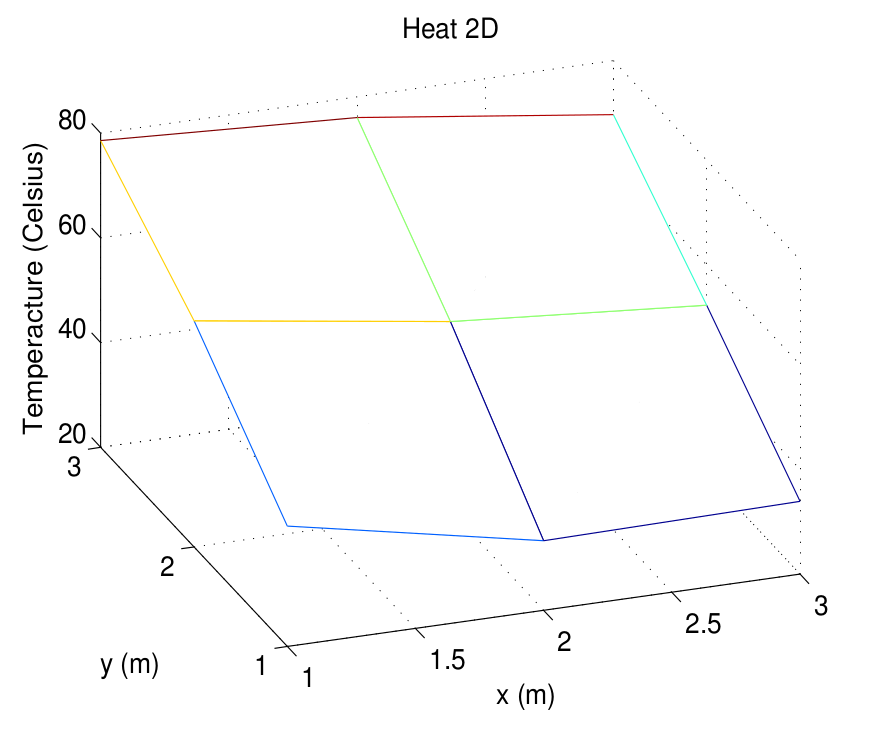
\includegraphics[height=0.4\textwidth,width=0.5\textwidth]{Graphics/Heat_Equation2D}
     \end{center}
   \end{figure}

\item {\bf Gauss-Seidel Method}

    Just as in the single dimensional heat equation the process of
    creating the matrices above is very tedious when performing this
    by hand. Thus it is beneficial to create a routine that can
    iterate until convergence. Taking equation \ref{e:heat_equation2d}
    and rearranging for $T_{i,j}$ yields 

    \begin{equation}
      T_{i,j} = (T_{i+1,j} + T_{i-1,j} + T_{i,j+1} + T_{i,j-1})/4
    \end{equation}
    
    This again can be easily implemented into a numerical solver just
    as before. The code has been left out so that the reader may
    attempt to create this code as an exercise however the error
    between the iterative solution and the solution from above even
    after 10 iterations is on the order of $10^-3$ as shown by the
    mesh plot of the error below. Of course this is specific to the
    initial guess but the iterative method is still robust to changes
    in grid size. This is known as the Gauss-Seidel Method.
    
    \begin{figure}[H]
     \begin{center}
       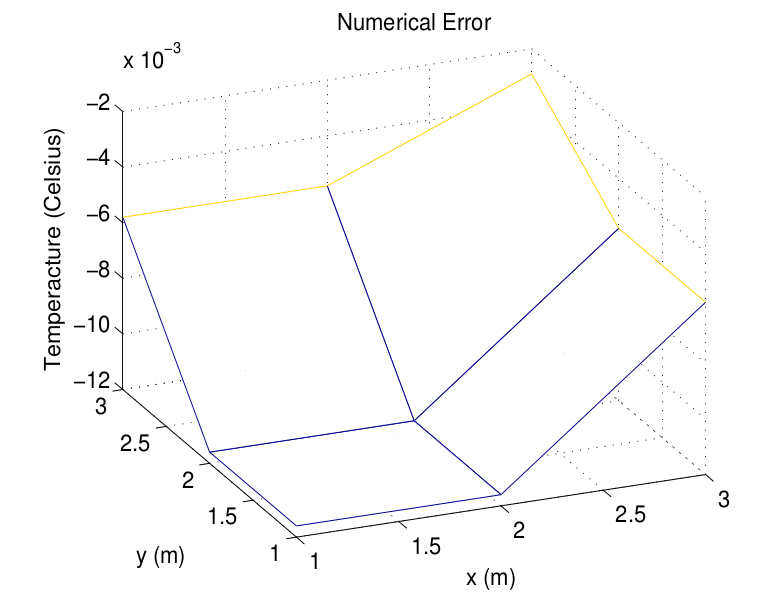
\includegraphics[height=0.4\textwidth,width=0.5\textwidth]{Graphics/Heat_Equation2D_Error}
     \end{center}
   \end{figure}    

  \item {\bf Derivative Boundary Conditions}

    If derivative boundary conditions are introduced we no longer have
    the value of T at the boundary. Instead we have the value of the
    derivative. In order to incorporate the derivative boundary the
    central difference equation is written for the boundary point such
    that

    \beq
    T_{1,j} + T_{-1,j} + T_{0,j+1} + T_{0,j-1} - 4 T_{0,j} = 0
    \eeq

    Notice that the variable $T_{-1,j}$ has been introduced which is
    outside the boundary. However this variable can be used to
    substitute the derivative into the finite difference equations.

    \beq
    \frac{\partial T_{0,j}}{\partial x} =
    \frac{T_{1,j}-T_{-1,j}}{2\Delta x}
    \eeq
    
    The equation above can be solved for $T_{-1,j}$ and substituted
    into the $0,j$ equation to yield

    \beq
    2T_{1,j} -2\Delta x \frac{\partial T_{0,j}}{\partial x} + T_{0,j+1} + T_{0,j-1} - 4 T_{0,j} = 0
    \eeq

    The equation above can be used for all nodes with a derivative
    boundary condition to solve for the heat flux in a plate.

    \item {\bf Vibrating String}

    Another elliptic equation is the vibrating string which can be
    solved in a similar fashion.

    \begin{equation}
      T \frac{\partial^2 v}{\partial x^2} - m \frac{\partial^2
        v}{\partial t^2} = 0
    \end{equation}

    In the equation above, T is the tension in the string and m is the mass per unit
    length of the rod. $v(x,t)$ is the amount of deflection in the
    string as a function of space and time. Notice that in this
    equation the time derivative is second order. Thus Euler's method
    is not accurate enough to compute the time derivative and a higher
    order method such as a Runge-Kutta-4 scheme must be used in order
    to converge to the solution.

  \item {\bf Parabolic Equations}

    An example parabolic equation is again a heat equation however
    here the equation is a function of x and time. The equation is
    given below

    \begin{equation}\label{e:parabolic}
      k\frac{\partial^2 T}{\partial x^2} = \frac{\partial T}{\partial t}
    \end{equation}

    Just as before the spatial derivative is approximated using
    central finite differencing however a superscript has been added
    to denote the time variable. That is $T_{1}^3$ is the value of
    temperature at the first node at time t = 3.

    \begin{equation}\label{e:spaceheat}
      \frac{T_{i+1}^l - 2T_{i}^l + T_{i-1}^l}{\Delta x^2} =
      \frac{\partial^2 T}{\partial x^2}
    \end{equation}

    Similarly Euler's Method can be used to approximate the time
    derivative of T.

    \begin{equation}\label{e:timeheat}
      \frac{\partial T}{\partial t} = \frac{T^{l+1}-T^l}{\Delta t}
    \end{equation}

    If equations \ref{e:timeheat} and \ref{e:spaceheat} are
    substituted in equation \ref{e:parabolic} and rearranged for
    $T_i^{l+1}$ the Finite Difference Method equation becomes    

    \begin{equation}
      T_i^{l+1} = T_i^l + \lambda (T_{i+1}^l - 2T_i^l + T_{i-1}^l)
    \end{equation}

    where $\lambda = \frac{k\Delta t}{\Delta x^2}$. Note, just like
    Euler's method, there are limits on stability for this method. In
    Carnahan et al. 1969 it was proved that the system is stable if
    $\Delta t \leq \frac{\Delta x^2}{2 k}$. The iterative method above
    thus combines the time dependent and spatially dependent portion
    of the rod. Thus, let us return to the simple static case we saw
    in section \ref{s:heat1D} where the rod is discretized into 6
    beads ($\Delta x = 2 m$ and L = 10 m) such that $T(0) = T_0 = 40$
    and $T(L) = T_5 = 200$. However, in this case let's assume that
    the rod has no heat at all except at the end points
     such that T = [200 0
     0 0 0 200]. The iterative procedure above is used to
    propogate the system forward to see how the heat in the rod
    evolves over time where $k' = 0.49 cal/(s-cm-^oC)$. Again the code
    has been removed and left for an exercise to the reader. The
    temperature distribution as a function of time is shown in the
    figure below.

    \begin{figure}[H]
      \begin{center}
       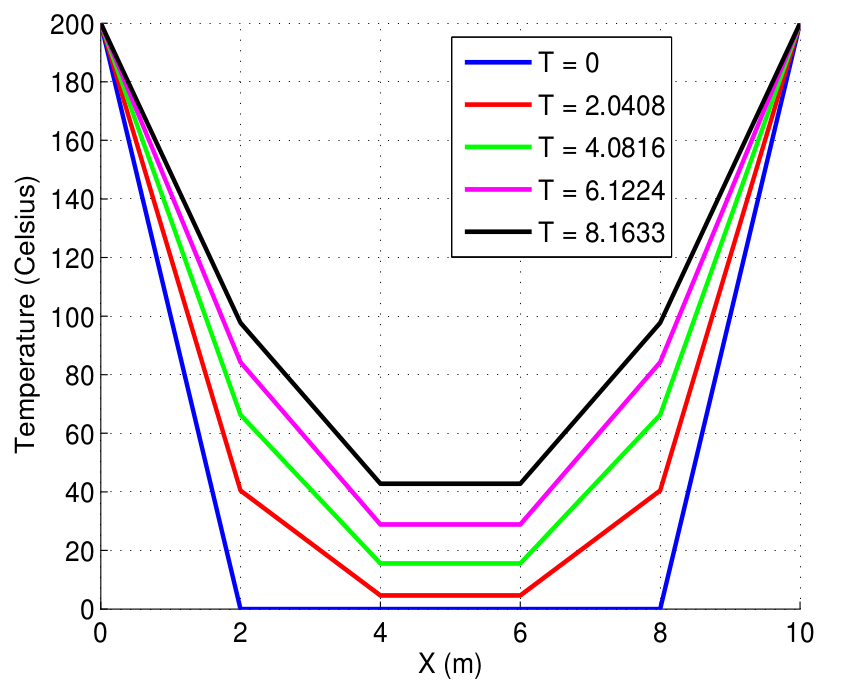
\includegraphics[height=0.4\textwidth,width=0.5\textwidth]{Graphics/Heat_Rod_Time}
      \end{center}
    \end{figure}

    This can also be visualized in three dimensions where a mesh plot
    is created. Here the x axis is the length of the rod, the y axis
    is the time variable and the z axis is the temperature along the
    rod. It is clear that the temperature in the rod is slowly heating
    up to $200^o C$.

    \begin{figure}[H]
      \begin{center}
        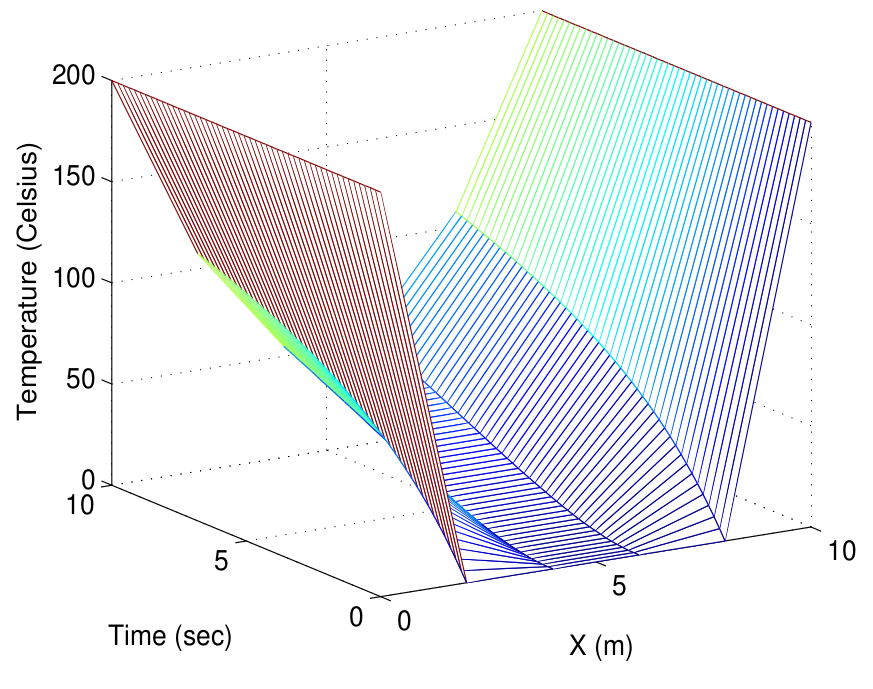
\includegraphics[height=0.4\textwidth,width=0.5\textwidth]{Graphics/Heat_Time_Mesh}
      \end{center}
    \end{figure}

  \item {\bf Crank-Nicolson Method}

    The Crank-Nicolson method is an implicit method rather than an
    explicit method. That is, rather than computing the next time step
    forward one at a time for each spatial coordinate, each timestep
    is computed simultaneously for the entire rod. The equations are
    obviously more complex however, it does not have the stability
    problem that the explicit method has because the spatial and time
    derivatives are second order accurate. First, the time derivative
    is approximated at the midpoint of time using the equation below.

    \beq
    \frac{\partial T}{\partial t} = \frac{T_i^{l+1}-T_i^l}{\Delta t}
    \eeq

    The spatial derivative is then approximated as an average of the
    forward point $l+1$ and the current time point $l$.

    \beq
     \frac{\partial^2 T}{\partial x^2} =
     \frac{1}{2}\left[\frac{T_{i+1}^l - 2T_{i}^l + T_{i-1}^l}{\Delta
         x^2} + \frac{T_{i+1}^{l+1} - 2T_{i}^{l+1} + T_{i-1}^{l+1}}{\Delta
         x^2} \right]
    \eeq

    Substituting these two equations into equation \ref{e:parabolic}
    results in

    \beq
    -\lambda T_{i-1}^{l+1} +2(1+\lambda) T_{i}^{l+1} - \lambda
    T_{i+1}^{l+1} = \lambda T_{i-1}^l + 2(1- \lambda)T_{i}^l + \lambda T_{i+1}^l
    \eeq

    where $\lambda = \frac{k\Delta t}{\Delta x^2}$. For the first
    point above $i=1$ the equation becomes

    \beq
    2(1+\lambda) T_{1}^{l+1} - \lambda
    T_{2}^{l+1} = \lambda T_{0}^l + \lambda T_{0}^{l+1} + 2(1- \lambda)T_{1}^l + \lambda T_{2}^l
    \eeq
    
    for the last point $i=m$, the equation becomes

    \beq
    -\lambda T_{m-1}^{l+1} +2(1+\lambda) T_{m}^{l+1}  = \lambda
    T_{m+1}^{l+1} + \lambda T_{m-1}^l + 2(1- \lambda)T_{m}^l + \lambda T_{m+1}^l
    \eeq
    
    where $T_0$ and $T_{m+1}$ are boundary conditions. These equations
    can be stacked in matrix form to yield the following equations.

    \beq
    \begin{bmatrix} 2(1+\lambda) & -\lambda & \hdots & 0 & 0 & 0 &
      \hdots & 0 & 0 \\ 0 & 0 & \hdots & -\lambda & 2(1+\lambda) &
      -\lambda & \hdots & 0 & 0 \\ 0 & 0 & \hdots & 0 & 0 & 0 &
      \hdots & -\lambda & 2(1+\lambda) \end{bmatrix} \begin{Bmatrix} T_1^{l+1}
      \\ T_2^{l+1} \\ \vdots \\ T_{i-1}^{l+1} \\ T_i^{l+1}
      \\ T_{i+1}^{l+1} \\ \vdots \\ T_{m-1}^{l+1}
      \\ T_m^{l+1} \end{Bmatrix} = \vec{b}
    \eeq

    where $\vec{b}$ is

    \beq
    \vec{b} = 
    \begin{Bmatrix} \lambda T_0^l +
      \lambda T_0^{l+1} + 2(1-\lambda) T_1^l + \lambda T_2^l \\ \vdots \\
      \lambda T_{i-1}^l + 2(1-\lambda) T_i^l + \lambda T_{i+1}^l
      \\ \vdots \\ \lambda T_{m-1}^l + \lambda T_{m+1}^{l+1} + 2(1-\lambda) T_m^l + \lambda
      T_{m+1}^l \end{Bmatrix}
    \eeq

    The assumption here is that every coordinate at $T^l$ is known and
    the equation above is used to compute the entire bar at the next
    timestep. In addition, the equation is of the form $A\vec{x} = \vec{b}$. 
    The solution to this equation is $A^{-1}\vec{b}$ however since the
    A matrix is constant this equation can be solved iteratively
    extremely quickly. 
    

\end{enumerate}
